\section{Results}
\label{sec:results}

Unless stated otherwise, bounds are for stage~D (width, thickness, strip angle, etch depth, rib angle, $\nsi$ and
$\nox$ unknown) with realistic priors, $\sigma_\lambda=\qty{1}{pm}$, at derivative step $h$, and ranges are over the
steps $h/2$, $h$ and $2h$. Bounds labelled ``ring and MZI'' include an MZI per structure. Table~\ref{tab:summary}
collects the main sets.

\begin{table}[!t]
\caption{Strip sidewall-angle CRLB $\sth$ for the main test-structure sets (stage~D, realistic priors). Ranges are
over the derivative steps $h/2$, $h$, $2h$; ``MC'' is the standard deviation of 2000 nonlinear fits at
\qty{1}{pm} (ring and MZI, surrogate model). One rib: strip TE rings at five widths plus a \qty{500}{nm} rib; two-width: the same strips plus ribs of \qty{300}{nm} and \qty{500}{nm}. The ring-only best set of eight has a different composition from the
ring-and-MZI one (Section~\ref{sec:multi}).}
\label{tab:summary}
\centering
\setlength{\tabcolsep}{2.5pt}
\begin{tabular}{@{}lccccc@{}}
\toprule
Set & \multicolumn{3}{c}{$\sth$ at \qty{1}{pm} (\si{\degree})} & \qty{0.1}{pm} & MC \\
 & ring & \multicolumn{2}{c}{ring and MZI} & (\si{\degree}) & (\si{\degree}) \\
 & only & $h$ & range & & \\
\midrule
Strips only (any) & $\infty$ & $\infty$ & -- & $\infty$ & -- \\
One rib (\qty{70}{nm}) & -- & 25.19 & -- & -- & -- \\
Two-width (\qty{50}{nm}) & 0.3932 & 0.3891 & 0.3891--0.3997 & 0.04077 & 0.3976 \\
Best set of 8 (\qty{90}{nm}) & 0.1895 & 0.139 & 0.1007--0.1473 & 0.0139 & 0.1323 \\
\bottomrule
\end{tabular}
\end{table}

\subsection{Strips are blind to the angle}

Fig.~\ref{fig:sections} shows the mechanism. For the strip the wall weight $W(y)$ is symmetric about mid-height and
its centroid sits at $y_c=t/2$. For the rib the weight is concentrated near the slab corner and the centroid lies below
the middle of the wall. The femwell derivatives follow~\eqref{eq:R}. Over all ten strips, in TE and TM and for both
$\neff$ and $\ngr$, the ratio $(\partial n/\partial\theta)/(\partial n/\partial w)$ lies between \qty{3.8396}{nm} and
\qty{3.8725}{nm} per degree, against $t\tan(\qty{1}{\degree})=\qty{3.8401}{nm}$; the largest deviation is
\qty{0.84}{\percent}. The closed-form $R$ computed from the mode-field centroid matches the femwell ratio within
\qty{0.79}{\percent} for the strips, a median of \qty{1.25}{\percent} for the ribs, and at worst \qty{5.4}{\percent}.
For ribs, $R$ lies between 0.831 and 0.873 on the \qty{50}{nm} slab and between 0.750 and 0.799 on the
\qty{90}{nm} slab, and it falls as the slab thickens (Fig.~\ref{fig:ratio}). With the symmetry imposed, the best set of
strips of any size from one to eight has an infinite bound.

\begin{figure*}[!t]
\centering
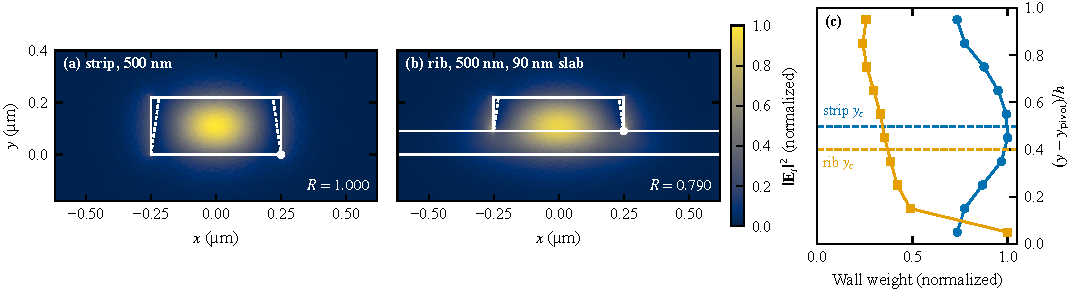
\includegraphics{fig1_sections}
\caption{Why a strip cannot see its sidewall angle. (a)~Oxide-clad strip, \qty{500}{nm}~$\times$~\qty{220}{nm}, and
(b)~rib, \qty{500}{nm} wide on a \qty{90}{nm} slab, both TE at $\lambda=\qty{1.55}{\micro m}$, with the transverse
intensity $|\mathbf{E}_t|^2$, the nominal wall (solid) and a tilted wall (dashed; \qty{8}{\degree}, exaggerated for
visibility) pivoting about the bottom corner (dot). The femwell angle/width ratio $R$ is printed in each panel.
(c)~First-order wall-perturbation weight $W$ along the right wall versus height above the pivot, normalized to its
maximum, with the centroids $y_c$ (dashed). The strip weight is symmetric about mid-height, so a tilt is exactly a width
change ($R=1$); the rib weight sits low on the wall, so $R<1$.}
\label{fig:sections}
\end{figure*}

\begin{figure}[!t]
\centering
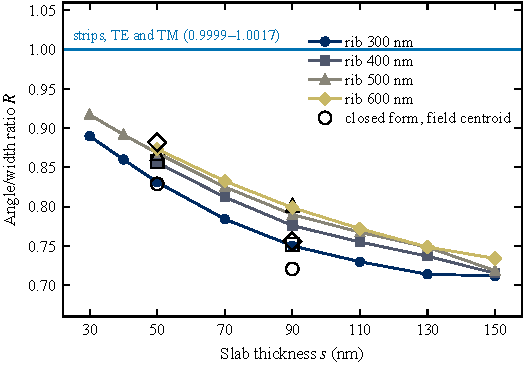
\includegraphics{fig2_ratio}
\caption{Angle/width ratio $R$ of the TE ribs versus slab thickness for four rib widths (femwell derivatives at step
$h$; $\lambda=\qty{1.55}{\micro m}$, $t=\qty{220}{nm}$, oxide-clad). Open symbols: closed form
$R=(y_c-y_\mathrm{pivot})/(h/2)$ from the mode field at the \qty{50}{nm} and \qty{90}{nm} slabs. The line at $R=1$ is
the strip value, set by symmetry. Every rib breaks the strip degeneracy, and thinner slabs break it least.}
\label{fig:ratio}
\end{figure}

\subsection{One rib against unknown etch parameters}

Fig.~\ref{fig:stages} follows a rib on a \qty{70}{nm} slab through the stages (ring and MZI). If the rib shares the
strip angle (stage~B) and only its depth is unknown, one rib width already gives \qty{0.357}{\degree} and two widths
give \qty{0.00365}{\degree}. When the rib has its own angle (stage~C), the single rib leaves the strip angle
unidentifiable, as the count in Section~\ref{sec:structures} predicts, while the two-width set gives
\qty{0.448}{\degree} without priors. Adding $\nsi$, $\nox$ (stage~D) and temperature (stage~E) moves the two-width
bound to \qty{0.481}{\degree} without priors and to \qty{0.452}{\degree} and \qty{0.455}{\degree} with realistic
priors.

\begin{figure}[!t]
\centering
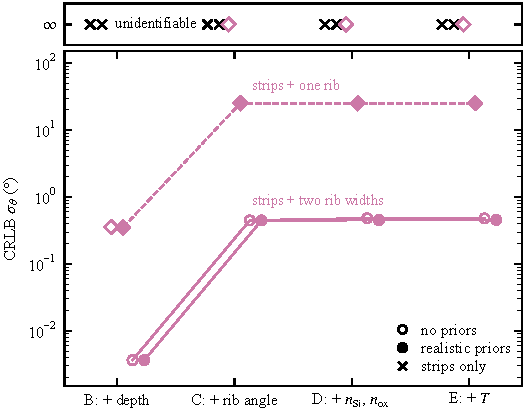
\includegraphics{fig3_stages}
\caption{Strip sidewall-angle CRLB as process unknowns are added (B: etch depth, rib angle tied to the strip angle;
C: separate rib angle; D: silicon and oxide indices; E: temperature), for strips alone (crosses), strips plus one
\qty{500}{nm} rib (diamonds) and strips plus ribs of \qty{500}{nm} and \qty{300}{nm} (circles), all on a \qty{70}{nm}
slab, without priors (open) and with realistic priors (filled), at $\sigma_\lambda=\qty{1}{pm}$, ring and MZI. Cases
with a singular Fisher matrix are drawn in the band marked $\infty$. A second width of the same rib keeps the angle
identifiable once the partial etch has its own angle.}
\label{fig:stages}
\end{figure}

With a single rib whose etch angle is independent of the strip's (stage~C, \qty{70}{nm} slab, \qty{1}{pm}), prior
knowledge improves the bound only partially. Realistic priors give $\sth=\qty{25.18}{\degree}$, knowing the etch depth to
\qty{0.01}{nm} (far beyond what a separate thickness measurement provides) gives \qty{5.03}{\degree}, and tying the rib
and strip angles to within \qty{1}{\degree} gives \qty{1.25}{\degree}. Two widths of the same rib reach
\qty{0.448}{\degree} at the same stage without any of these assumptions. In stage~D with realistic priors, the single
rib gives between \qty{24.4}{\degree} and \qty{45.4}{\degree} depending on the slab, values set by the priors.

\subsection{Multi-width rib sets}
\label{sec:multi}

The two-width set consists of strip TE rings at the five widths plus ribs of \qty{300}{nm} and \qty{500}{nm} on a
\qty{50}{nm} slab. Read by rings alone it gives $\sth=\qty{0.3932}{\degree}$; with an MZI per structure it gives
\qty{0.3891}{\degree} (\qtyrange{0.3891}{0.3997}{\degree} over steps). It is insensitive to derivative errors. On a
fixed mesh the bound (ring and MZI) is \qty{0.394}{\degree}, a \qty{1.3}{\percent} change, and random errors of
$\pm\qty{0.3}{\percent}$ on every \qty{300}{nm}-rib derivative spread it only between \qty{0.364}{\degree} and
\qty{0.420}{\degree} (5th to 95th percentile).

The exhaustive search finds lower bounds with more rib widths and some TM strips. Among ring-only sets, the best set
of eight (TE strips of 400, 550 and \qty{600}{nm}, a TM strip of \qty{400}{nm}, and ribs of 300, 400, 500 and
\qty{600}{nm} on a \qty{90}{nm} slab) gives \qty{0.1895}{\degree}, and the best sets of four to seven give 0.4356,
0.3606, 0.2029 and \qty{0.1941}{\degree}. With an MZI per structure, the best set of eight (TE and TM strips of
\qty{400}{nm} and \qty{600}{nm} and the same four ribs) gives $\sth=\qty{0.139}{\degree}$
(\qtyrange{0.101}{0.147}{\degree} over steps). This set is more sensitive to derivative accuracy than the two-width
set. With fixed-mesh derivatives for the \qty{300}{nm} rib its bound becomes \qty{0.118}{\degree}
(\qty{-15.3}{\percent}), the fixed-mesh and remeshed derivatives differing by at most \qty{0.78}{\percent}, and random
$\pm\qty{0.3}{\percent}$ errors spread it between \qty{0.109}{\degree} and \qty{0.189}{\degree}. We therefore quote
\qtyrange{0.12}{0.14}{\degree} for it, with a derivative-accuracy uncertainty of about \qty{15}{\percent}.

A greedy search that adds one structure at a time reached the exhaustive optimum in 25 of the 32 stage, prior and slab
cases we compared and fell short in 7, with a bound up to a factor of 1.12 larger. At the best-case \qty{0.1}{pm}
precision both ring-and-MZI bounds shrink tenfold, to \qty{0.0408}{\degree} for the two-width set and
\qty{0.0139}{\degree} for the best set. They scale linearly with $\sigma_\lambda$ (\qty{0.196}{\degree} and
\qty{0.775}{\degree} for the two-width set at 0.5 and \qty{2}{pm}).

\subsection{Ring and MZI readout}
\label{sec:mzi}

For the two-width set, adding an MZI per structure lowers the bound from \qty{0.3932}{\degree} (rings only) to
\qty{0.3891}{\degree}. If the MZI phase is three times noisier than our derived value, the bound is
\qty{0.3925}{\degree}; at ten times it is \qty{0.3932}{\degree}, the ring-only value. For the best set of eight the
MZI matters more, \qty{0.1901}{\degree} without it and \qty{0.1390}{\degree} with it, but a threefold noisier MZI
already gives \qty{0.1815}{\degree}. The MZI gain therefore depends on locating a broad fringe as precisely as a narrow
resonance, an assumption we cannot support from the literature, and we base the proposal on rings.

\subsection{Monte Carlo fits reach the bound}

\begin{figure*}[!t]
\centering
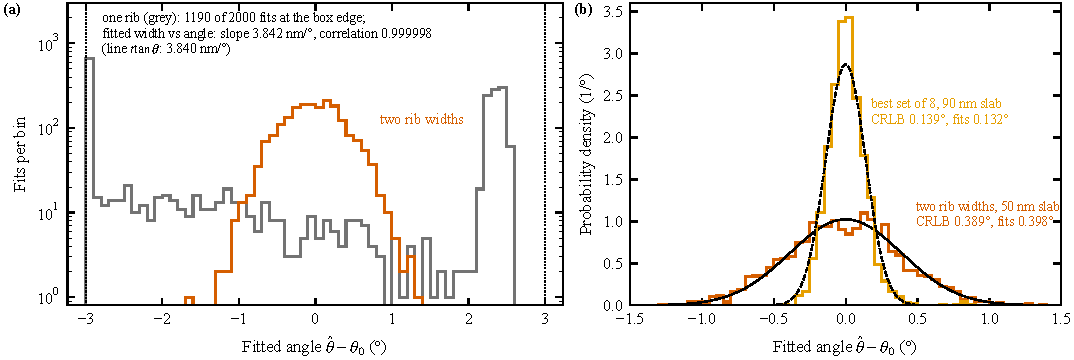
\includegraphics{fig4_montecarlo}
\caption{Monte Carlo fits of 2000 simulated noisy measurement sets per set at $\sigma_\lambda=\qty{1}{pm}$
(stage~D, realistic priors, ring and MZI, bounded nonlinear least squares on the surrogate model). (a)~Histograms of
the fitted strip angle for strip TE rings at five widths plus one \qty{500}{nm} rib (grey) and plus ribs of
\qty{300}{nm} and \qty{500}{nm} (orange), both on a \qty{50}{nm} slab; dotted lines mark the $\pm\qty{3}{\degree}$ fit
box. With one rib the fits spread over the whole box along the width/angle valley. (b)~Fitted-angle histograms for the
two-width set and the best set of eight (\qty{90}{nm} slab) with Gaussians of the CRLB width (lines). With two or more
rib widths the fit scatter matches the bound.}
\label{fig:mc}
\end{figure*}

Fig.~\ref{fig:mc} compares the nonlinear fits with the bound. For the two-width set the fitted angles have a standard
deviation of \qty{0.398}{\degree} (\qtyrange{0.385}{0.410}{\degree}, 95\% bootstrap interval), 1.02 times the CRLB,
with a bias of \qty{-0.015 \pm 0.0089}{\degree}; none of the 2000 fits failed, ended ambiguous or reached the box edge.
For the best set the spread is \qty{0.132}{\degree} (\qtyrange{0.125}{0.140}{\degree}), 0.952 times the CRLB, with a
bias of \qty{0.0075 \pm 0.003}{\degree}; 4 fits ended at the box edge and none failed. The spread is slightly below the
femwell CRLB because the surrogate's own bound at nominal is \qty{0.1249}{\degree}; its \qty{300}{nm}-rib slopes are a
smooth fit through the remeshing scatter. With one rib the fits find the valley predicted by the symmetry argument. The
linearized bound is \qty{29.52}{\degree}, so the $\pm\qty{3}{\degree}$ fit box confines the estimates, and the data do
not: 1190 of the 2000 fits end at the edge of the box, 12 are ambiguous and 20 fail. The fitted widths and angles lie
on a line of slope \qty{3.842}{nm} per degree with a correlation of 0.999998, against
$t\tan(\qty{1}{\degree})=\qty{3.8401}{nm}$ (Fig.~\ref{fig:mc}(a)).

% numbers from results_review/data/surrogate_check.json (HEADLINE_NUMBERS.md section P)
\subsection{Monte Carlo on femwell data}
\label{sec:surrcheck}

The fits above take both the data and the model from the surrogate, so they cannot show what the surrogate's own
errors do to the estimate. For each of the two sets we drew 20 parameter vectors from the CRLB covariance, solved
every structure at each of them with femwell on the r12 mesh (160 solves for the best set, 140 for the two-width set),
and used these mode indices as noiseless data. Each data set received 25 noise realizations at
\qty{1}{pm}, giving 500 fits per set, all made with the surrogate as the model and the settings above.

At these geometries the surrogate follows the strips to within $0.8627\,\sigma_\phi$ in $\neff$, and its $\ngr$ errors
stay below $0.0524\,\sigma_{\ngr}$. The \qty{300}{nm} ribs are again the weak point. On the \qty{50}{nm} slab their
$\neff$ misses femwell by $5.166\,\sigma_\phi$ RMS and by $12.42\,\sigma_\phi$ at worst, and on the \qty{90}{nm} slab
by $1.519\,\sigma_\phi$ and $3.366\,\sigma_\phi$.

The two-width set does not pass these errors on to the angle. Its fitted angles scatter by \qty{0.4034}{\degree}
(\qtyrange{0.3781}{0.4273}{\degree}, 95\% bootstrap interval), 1.037 times the CRLB, with a mean error of
\qty{0.02463 \pm 0.01804}{\degree}, and all 500 fits converge inside the box. The best set of eight does not reach its
bound on femwell data. Its spread is \qty{0.2067}{\degree} (\qtyrange{0.1859}{0.2253}{\degree}), 1.487 times the
CRLB of \qty{0.139}{\degree}, and 14 fits end at the box edge, even though the surrogate errors on its
\qty{300}{nm} rib are the smaller of the two. Its bound rests on small differences between four rib widths, and model
errors of about one noise standard deviation in one of them are enough to widen the estimate. The derivative checks
of Section~\ref{sec:multi} and the variation analysis of Section~\ref{sec:variation} show the same sensitivity. We
take \qty{0.39}{\degree} for the two-width set as the result that holds with an independent forward model, and the
\qty{0.139}{\degree} of the best set as the bound of a model accurate to better than the noise.


\subsection{Slab thickness}

For the ring-only two-width set the bound depends strongly on the slab (Fig.~\ref{fig:slab}). It is lowest at
\qty{50}{nm} (\qty{0.3932}{\degree}), rises slowly toward thinner slabs, to \qty{0.4079}{\degree} at \qty{40}{nm} and
\qty{0.4202}{\degree} at \qty{30}{nm}, and rises quickly toward thicker ones, to \qty{0.6001}{\degree} at \qty{90}{nm} and
\qty{4.094}{\degree} at \qty{150}{nm}. With an MZI the values are within \qty{1}{\percent} of these
(\qty{0.389}{\degree}, \qty{0.403}{\degree}, \qty{0.414}{\degree}, \qty{0.597}{\degree} and \qty{4.089}{\degree}).
Among the slabs simulated the optimum is therefore \qty{50}{nm}. Thinner slabs bring $R$ closer to 1
(Fig.~\ref{fig:ratio}), but we have not separated that effect from the other ways the slab changes the two rib modes.

\begin{figure}[!t]
\centering
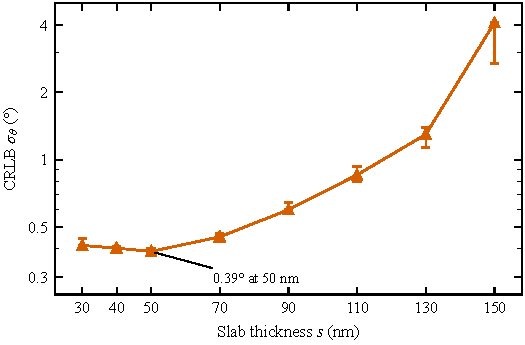
\includegraphics{fig5_slab}
\caption{CRLB of the two-width set (strip TE rings at 400--\qty{600}{nm} plus ribs of \qty{300}{nm} and
\qty{500}{nm}) versus slab thickness, stage~D, realistic priors, $\sigma_\lambda=\qty{1}{pm}$, ring and MZI,
$\lambda=\qty{1.55}{\micro m}$. Bars span the derivative steps $h/2$, $h$, $2h$. The bound is lowest at \qty{50}{nm}
and grows tenfold by \qty{150}{nm}.}
\label{fig:slab}
\end{figure}

\subsection{Measurement-model variants}
\label{sec:noise}

Fig.~\ref{fig:noise} shows how the two headline sets (ring and MZI) respond to departures from the baseline noise
model. A correlation between the $\neff$ and $\ngr$ errors of a ring lowers the bound. At the derived
$\rho=-1/\sqrt2$ the two-width set gives \qty{0.3365}{\degree} and the best set \qty{0.1142}{\degree}, and at
$\rho=0.9$ they give \qty{0.2996}{\degree} and \qty{0.0795}{\degree}. Treating the errors as independent is therefore
conservative.

A wavelength-calibration offset common to all rings matters for the two-width set. Left unknown, it raises the
two-width bound to \qty{1.070}{\degree}; known to \qty{10}{pm}, it gives \qty{0.3892}{\degree}, the baseline. The best
set barely notices the offset (\qty{0.1393}{\degree} unknown). The two-width set therefore needs an absolute
wavelength reference good to about \qty{10}{pm}.

Temperature as a shared unknown changes little. With a prior of \qty{1}{K} the two-width bound is
\qty{0.3917}{\degree}, and with no prior \qty{0.4122}{\degree}; the best set stays at \qty{0.1390}{\degree}. An
independent temperature drift of each structure between its readouts is more damaging. At \qty{10}{mK} per structure the
two-width set gives \qty{0.3935}{\degree} and the best set \qty{0.1877}{\degree}, and at \qty{100}{mK} they give
\qty{0.4599}{\degree} and \qty{0.4993}{\degree}. Larger, multi-structure sets therefore need tighter
thermal control.

\begin{figure}[!t]
\centering
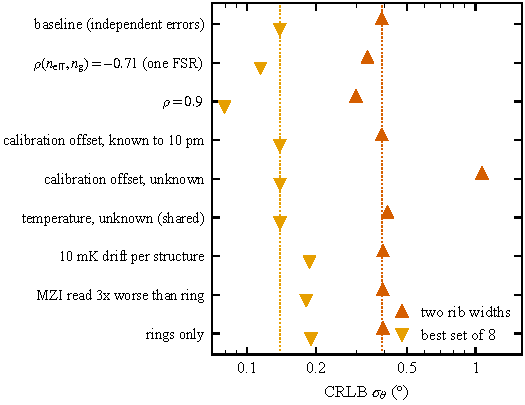
\includegraphics{fig7_noise}
\caption{Strip-angle CRLB of the two-width set (up triangles) and the best set of eight (down triangles) under variants
of the measurement model: stage~D, realistic priors, \qty{1}{pm}, ring and MZI unless the row states otherwise. Dotted
lines mark the baselines. Correlated ring errors lower the bound; an unknown calibration offset harms only the
two-width set; per-structure temperature drift and a noisier MZI harm mainly the best set.}
\label{fig:noise}
\end{figure}

\subsection{Departures from shared process parameters}
\label{sec:variation}

Every bound so far assumes that all structures in a set share one width offset, one thickness and one angle per etch.
A departure common to all structures is absorbed into these parameters. Departures that differ between structures are
not, and the fit converts them into a strip-angle error. For the two-width set the root-mean-square bias gain is
\qty{219.7}{\degree} of strip-angle bias per degree of independent per-structure angle offset, and \qty{57.62}{\degree}
per nanometre of independent width offset; for the best set the gains are \qty{194.1}{\degree} and \qty{74.41}{\degree}.
Per-structure angle offsets with a standard deviation of \qty{0.25}{\degree} thus bias the two-width estimate by
\qty{54.92}{\degree} (standard deviation), and width offsets of \qty{0.5}{nm} bias it by \qty{28.81}{\degree}. An
angle that changes linearly with waveguide width, by \qty{0.25}{\degree} per \qty{100}{nm}, biases the two-width
estimate by \qty{6.869}{\degree} and the best set by \qty{-36.93}{\degree}. Under such departures the shared-parameter
fit returns no useful angle.

If the departures are modeled as unknowns with a Gaussian prior (a random-effects model), the fit stays unbiased and
the bound grows instead (Fig.~\ref{fig:variation}). For the two-width set, per-structure angle departures of
\qty{0.01}{\degree} raise the bound to \qty{0.5502}{\degree}, and \qty{0.1}{\degree} raises it to \qty{2.295}{\degree};
width departures of \qty{0.1}{nm} raise it to \qty{1.139}{\degree}, and thickness departures of \qty{0.1}{nm} to
\qty{2.544}{\degree}. The bound doubles at a per-structure spread of \qty{0.01749}{\degree} in angle,
\qty{0.03938}{nm} in width or \qty{0.01705}{nm} in thickness. The best set is about ten times less tolerant. Its bound doubles at
\qty{0.001739}{\degree} in angle and \qty{0.00365}{nm} in width, and in thickness already below the smallest spread we
evaluated (\qty{0.001}{nm}). The extra structures that make the best set precise are the ones whose small differences the
fit cannot tell apart from the angle.

\begin{figure*}[!t]
\centering
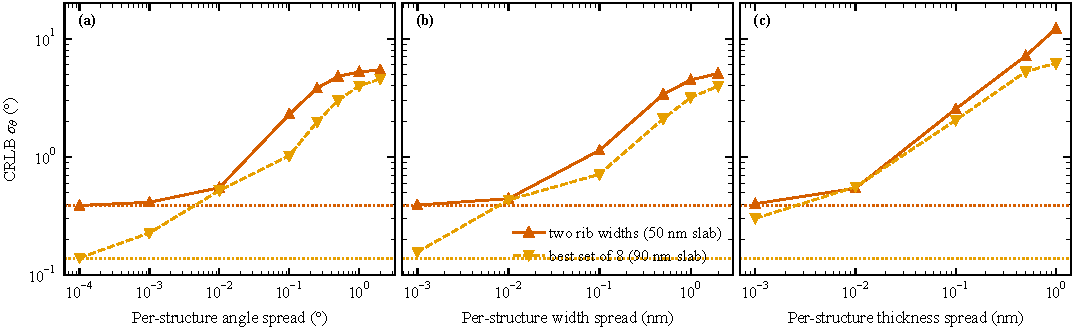
\includegraphics{fig6_variation}
\caption{Strip-angle CRLB when each structure may depart from the shared process parameters (random-effects model),
versus the per-structure spread of (a)~the sidewall angle, (b)~the width and (c)~the thickness, for the two-width set
and the best set of eight (stage~D, realistic priors, \qty{1}{pm}, ring and MZI). Dotted lines: shared-parameter CRLB.
The bound doubles at spreads of a few hundredths of a nanometre or degree for the two-width set, and ten times less for
the best set.}
\label{fig:variation}
\end{figure*}

\subsection{Resonance prediction}
\label{sec:prediction}

When strip rings are fitted with the angle held at its nominal value, a real \qty{1}{\degree} tilt is absorbed as a width
change of \qty{-3.84}{nm}. Using that width to predict a \qty{500}{nm} rib ring on a \qty{90}{nm} slab, whose angle
sensitivity differs ($R<1$), mispredicts its resonance by $\delta\lambda=\lambda\,\delta\neff/\ngr=\qty{-710.8}{pm}$ per
degree of unmodeled tilt.

With the angle in the model, the question becomes how well the extracted parameters predict other devices on the same
chip. We propagate the full parameter covariance of the two-width set to the resonance of a ring, using
$\sigma_{\lambda,\mathrm{pred}}=\lambda\sqrt{\mathbf{g}^{\mathsf T}\mathbf{C}\mathbf{g}}/\ngr$, where $\mathbf{g}$ is the
gradient of the device's $\neff$ and $\mathbf{C}$ is the inverse Fisher matrix. At \qty{1}{pm}, a strip TE ring of
\qty{500}{nm} is predicted to \qty{0.457}{pm} and a rib ring of \qty{500}{nm} on the \qty{50}{nm} slab to
\qty{0.773}{pm}. The angle uncertainty alone would give hundreds of picometres, but it is correlated with the width and
thickness uncertainties, and the combination that sets the resonance is well determined. With an unknown calibration
offset the prediction degrades to \qty{982.2}{pm}, because the two-width set cannot separate the offset from the
process parameters. For the best set the two devices are predicted to \qty{0.559}{pm} and, for the rib on its
\qty{90}{nm} slab, \qty{0.521}{pm}; with the offset unknown the strip ring is predicted to \qty{39.68}{pm}.
